\documentclass[a4paper]{article}
\usepackage[T1]{fontenc}			% \chapter package
\usepackage[english]{babel}
\usepackage[english]{isodate}  		% date format
\usepackage{graphicx}				% manage images
\usepackage{amsfonts}
\usepackage{booktabs}				% high quality tables
\usepackage{amsmath}				% math package
\usepackage{amssymb}				% another math package (e.g. \nexists)
\usepackage{bm}                     % bold math symbols
\usepackage{mathtools}				% emphasize equations
\usepackage{stmaryrd} 				% '\llbracket' and '\rrbracket'
\usepackage{amsthm}					% better theorems
\usepackage{enumitem}				% manage list
\usepackage{pifont}					% nice itemize
\usepackage{cancel}					% cancel math equations
\usepackage{caption}				% custom caption
\usepackage[]{mdframed}				% box text
\usepackage{multirow}				% more lines in a table
\usepackage{textcomp, gensymb}		% degree symbol
\usepackage[x11names]{xcolor}		% RGB color
\usepackage[many]{tcolorbox}		% colorful box
\usepackage{multicol}				% more rows in a table (used for the lists)
\usepackage{listings}
\usepackage{url}
\usepackage{qrcode}
\usepackage{fontawesome5}
\usepackage{ragged2e}
\usepackage{cite}                   % references
\usepackage{imakeidx}               % index
\makeindex[program=makeindex, columns=1,
           title=Index, 
           intoc,
           options={-s index-style.ist}]
\usepackage{fancyhdr}

%\pdfcompresslevel=0
%\pdfobjcompresslevel=0

\definecolor{codegreen}{rgb}{0,0.6,0}
\definecolor{codegray}{rgb}{0.5,0.5,0.5}
\definecolor{codepurple}{rgb}{0.58,0,0.82}
\definecolor{backcolour}{rgb}{0.95,0.95,0.92}
\lstdefinestyle{mystyle}{
    backgroundcolor=\color{backcolour},
    commentstyle=\color{codegreen},
    keywordstyle=\color{magenta},
    numberstyle=\tiny\color{codegray},
    stringstyle=\color{codepurple},
    basicstyle=\ttfamily\footnotesize,
    breakatwhitespace=false,
    breaklines=true,
    captionpos=b,
    keepspaces=true,
    numbers=left,
    numbersep=5pt,
    showspaces=false,
    showstringspaces=false,
    showtabs=false,
    tabsize=2
}
\lstset{style=mystyle}


% thanks Mico: https://tex.stackexchange.com/a/60218/312896
\makeatletter
\renewcommand\paragraph{\@startsection{paragraph}{4}{\z@}%
            {-2.5ex\@plus -1ex \@minus -.25ex}%
            {1.25ex \@plus .25ex}%
            {\normalfont\normalsize\bfseries}}
\makeatother
\setcounter{secnumdepth}{4} % how many sectioning levels to assign numbers to
\setcounter{tocdepth}{4}    % how many sectioning levels to show in ToC


% draw a frame around given text
\newcommand{\framedtext}[1]{%
	\par%
	\noindent\fbox{%
		\parbox{\dimexpr\linewidth-2\fboxsep-2\fboxrule}{#1}%
	}%
}


% table of content links
\usepackage{xcolor}
\usepackage[linkcolor=black, citecolor=blue, urlcolor=cyan]{hyperref} % hypertexnames=false
\hypersetup{
	colorlinks=true
}


\newtheorem{theorem}{\textcolor{Red3}{\underline{Theorem}}}
\renewcommand{\qedsymbol}{QED}
\newcommand{\dquotes}[1]{``#1''}
\newcommand{\longline}{\noindent\rule{\textwidth}{0.4pt}}
\newcommand{\circledtext}[1]{\raisebox{.5pt}{\textcircled{\raisebox{-.9pt}{#1}}}}
\newcommand{\definition}[1]{\textcolor{Red3}{\textbf{#1}}\index{#1}}
\newcommand{\definitionWithSpecificIndex}[2]{\textcolor{Red3}{\textbf{#1}}\index{#2}}
\newcommand{\example}[1]{\textcolor{Green4}{\textbf{#1}}}
\newcommand{\highspace}{\vspace{1.2em}\noindent}
\newcommand{\vectorNormSymbol}{\left|\left|\cdot\right|\right|}
\newcommand{\version}{v0.2.0-dev}
\newcommand{\nnz}{\mathrm{nnz}} % non-zero entries


\begin{document}
    \newcounter{definition}[section]
    \newcounter{example}[section]
    \newcounter{exercise}[section]
    
    \newtcolorbox[use counter = definition]{definitionbox}[1][]{%
        breakable,
        enhanced,
        colback=red!5!white,
        colframe=red!75!black,
        fonttitle=\bfseries,
        title={Definition \thetcbcounter#1} %
    }

    \newtcolorbox[use counter = exercise]{exercisebox}[1][]{%
        breakable,
        enhanced,
        colback=Red3!5!white,
        colframe=Red3!75!black,
        fonttitle=\bfseries,
        title={Exercise \thetcbcounter#1} %
    }
    
    \newtcolorbox[use counter = example]{examplebox}[1][]{%
        breakable,
        enhanced,
        colback=Green4!5!white,
        colframe=Green4!75!black,
        fonttitle=\bfseries,
        title={Example \thetcbcounter#1} %
    }

    \newtcolorbox[]{deepeningbox}[1][]{%
        breakable,
        enhanced,
        colback=DarkOrange3!5!white,
        colframe=DarkOrange3!75!black,
        fonttitle=\bfseries,
        title={Deepening#1} %
    }

    %%%%%%%%%%%%%%%
    % Notes cover %
    %%%%%%%%%%%%%%%
    \author{260236}
\title{Parallel Computing - Notes - \version}
\date{\printdayoff\today}
\maketitle

    %%%%%%%%%%%
    % Preface %
    %%%%%%%%%%%
	\section*{Preface}

Every theory section in these notes has been taken from the sources:
\begin{itemize}
    \item Course slides.\cite{numerical-linear-algebra-polimi}
\end{itemize}
About:
\begin{itemize}
    \item[\faIcon{github}] \href{https://github.com/PoliMI-HPC-E-notes-projects-AndreVale69/HPC-E-PoliMI-university-notes}{GitHub repository}
    \begin{center}
        \qrcode{https://github.com/PoliMI-HPC-E-notes-projects-AndreVale69/HPC-E-PoliMI-university-notes}
    \end{center}
\end{itemize}
These notes are an unofficial resource and shouldn't replace the course material or any other book on numerical linear algebra. It is not made for commercial purposes. I've made the following notes to help me improve my knowledge and maybe it can be helpful for everyone.

As I have highlighted, a student should choose the teacher's material or a book on the topic. These notes can only be a helpful material.

\highspace

\subsection*{Correlated Projects}

During the Numerical Linear Algebra for HPC course, I was part of a team where we created a project that included two challenges related to the course. See more details in the corresponding repository:
\begin{itemize}
    \item[\faIcon{github}] \href{https://github.com/PoliMI-HPC-E-notes-projects-AndreVale69/NLA-challenges}{GitHub repository}
    \begin{center}
        \qrcode{https://github.com/PoliMI-HPC-E-notes-projects-AndreVale69/NLA-challenges}
    \end{center}
\end{itemize}

    %%%%%%%%%%%%%%%%%%%%%
    % Table of contents %
    %%%%%%%%%%%%%%%%%%%%%
    \tableofcontents
    \newpage

    %%%%%%%%%%%%%%%%%%%
    % Fancy pagestyle %
    %%%%%%%%%%%%%%%%%%%
    \pagestyle{fancy}
    \fancyhead{} % clear all header fields
    \fancyhead[R]{\nouppercase{\leftmark\hfill\rightmark}}
    
    %%%%%%%%%%%%%%%%%
    % Preliminaries %
    %%%%%%%%%%%%%%%%%
    \section{Preliminaries}

This section introduces some of the basic topics used throughout the course.

\subsection{Notation}

    \subsection{Matrix Operations}

Some basic matrix operations:
\begin{itemize}
	\item \textbf{Inner products}. If $\mathbf{x}, \mathbf{y} \in \mathbb{R}^{n}$ then:
	\begin{equation*}
		\mathbf{x}^{T} \mathbf{y} = \displaystyle\sum_{i = 1, \dots, n} x_{i}y_{i}
	\end{equation*}
	For real vectors, the commutative property is true:
	\begin{equation*}
		\mathbf{x}^{T} \mathbf{y} = \mathbf{y}^{T} \mathbf{x}
	\end{equation*}
	Furthermore, the vectors $\mathbf{x}, \mathbf{y} \in \mathbb{R}^{n}$ are \textbf{orthogonal} if:\index{Orthogonal Vectors}
	\begin{equation*}
		\mathbf{x}^{T} \mathbf{y} = \mathbf{y}^{T} \mathbf{x} = \mathbf{0}
	\end{equation*}
	And finally, some useful properties of matrix multiplication:
	\begin{enumerate}
		\item Multiplication by the \emph{identity} changes nothing.
		\begin{equation*}\index{Matrices Multiplication}
			A \in \mathbb{R}^{n \times m} \: \Rightarrow \: \mathbf{I}_{n} A = A = A\mathbf{I}_{m}
		\end{equation*}
		
		\item Associativity:
		\begin{equation*}\index{Matrix Associativity Property}
			A\left(BC\right) = \left(AB\right)C
		\end{equation*}
		
		\item Distributive:
		\begin{equation*}\index{Matrix Distributive Property}
			A\left(B+D\right) = AB + AD
		\end{equation*}
		
		\item \underline{No} commutativity:
		\begin{equation*}
			AB \ne BA
		\end{equation*}
		
		\item Transpose of product:
		\begin{equation*}\index{Transpose product between matrices}
			\left(AB\right)^{T} = B^{T} A^{T}
		\end{equation*}
	\end{enumerate}
	
	\item \textbf{Matrix powers}. For $A \in \mathbb{R}^{n \times n}$ with $A \ne \mathbf{0}$:
	\begin{equation*}
		A^{0} = \mathbf{I}_{n} \hspace{2em} A^{k} = \underbrace{A \cdots A}_{k\text{ times}} = AA^{k-1} \hspace{2em} k \ge 1
	\end{equation*}
	Furthermore, $A \in \mathbb{R}^{n \times n}$ is:
	\begin{itemize}
		\item \textbf{Idempotent} (projector) $A^{2} = A$ \index{Idempotent Matrices}
		\item \textbf{Nilpotent} $A^{k} = \mathbf{0}$ for some integer $k \ge 1$ \index{Nilpotent Matrices}
	\end{itemize}
	
	\item \textbf{Inverse}. For $A \in \mathbb{R}^{n \times n}$ is \definitionWithSpecificIndex{non-singular}{Non-singular Matrices} (\definitionWithSpecificIndex{invertible}{Invertible Matrices}), if exists $A^{-1}$ with:
	\begin{equation}\label{eq: non-singular matrix}
		AA^{-1} = \mathbf{I}_{n} = A^{-1}A
	\end{equation}
	Inverse and transposition are interchangeable:
	\begin{equation*}
		A^{-T} \triangleq \left(A^{T}\right)^{-1} = \left(A^{-1}\right)^{T}
	\end{equation*}
	Furthermore, an inverse of a product for a matrix $A \in \mathbb{R}^{n \times n}$ can be expressed as:
	\begin{equation*}
		\left(AB\right)^{-1} = B^{-1}A^{-1}
	\end{equation*}
	Finally, remark that if $\mathbf{0} \ne \mathbf{x} \in \mathbb{R}^{n}$ and $A\mathbf{x} = 0$, then $A$ is \definitionWithSpecificIndex{singular}{Singular Matrices}.
	
	\item \textbf{Orthogonal matrices}. Given a matrix $A \in \mathbb{R}^{n \times n}$ that is \emph{invertible}, the matrix $A$ is said to be \definitionWithSpecificIndex{orthogonal}{Orthogonal Matrices} if:
	\begin{equation*}
		A^{-1} = A^{T} \: \Rightarrow \: A^{T}A = \mathbf{I}_{n} = AA^{T}
	\end{equation*}
	
	\item \textbf{Triangular matrices}. There are two types of triangular matrices:
	\begin{enumerate}
		\item \definition{Upper triangular matrix}:
		\begin{equation*}
			\mathbf{U} = \begin{bmatrix}
				u_{1,1} & u_{1,2} & \cdots & u_{1,n} \\
				0 & u_{2,2} & \cdots & u_{2,n} \\
				\vdots & \cdots & \ddots & \vdots \\
				0 & 0 & \cdots & u_{n,n} \\
			\end{bmatrix}
		\end{equation*}
		$\mathbf{U}$ is \textbf{non-singular} if and only if $u_{ii} \ne 0$ for $i = 1, \dots, n$.

		\item \definition{Lower triangular matrix}:
		\begin{equation*}
			\mathbf{L} = \begin{bmatrix}
				l_{1,1} & 0 & \cdots & 0 \\
				l_{2,1} & l_{2,2} & \cdots & 0 \\
				\vdots & \cdots & \ddots & \vdots \\
				l_{n,1} & l_{n,2} & \cdots & l_{n,n} \\
			\end{bmatrix}
		\end{equation*}
		$\mathbf{L}$ is \textbf{non-singular} if and only if $l_{ii} \ne 0$ for $i = 1, \dots, n$.
	\end{enumerate}
	
	\item \textbf{Unitary triangular matrices}. Are matrices similar to the lower and upper matrices, but they have the main diagonal composed of ones.
	\begin{enumerate}
		\item \definition{Unitary upper triangular matrix}:
		\begin{equation*}
			\mathbf{U} = \begin{bmatrix}
				1 & u_{1,2} & \cdots & u_{1,n} \\
				0 & 1 & \cdots & u_{2,n} \\
				\vdots & \cdots & \ddots & \vdots \\
				0 & 0 & \cdots & 1 \\
			\end{bmatrix}
		\end{equation*}

		\item \definition{Unitary lower triangular matrix}:
		\begin{equation*}
			\mathbf{L} = \begin{bmatrix}
				1 & 0 & \cdots & 0 \\
				l_{2,1} & 1 & \cdots & 0 \\
				\vdots & \cdots & \ddots & \vdots \\
				l_{n,1} & l_{n,2} & \cdots & 1 \\
			\end{bmatrix}
		\end{equation*}
	\end{enumerate}
\end{itemize}
    \subsection{Basic matrix decomposition}

In the Numerical Linear Algebra course, we will use three main decomposition:
\begin{itemize}
	\item \underline{\textbf{LU factorization with (partial) pivoting}}. If $A \in \mathbb{R}^{n \times n}$ is a non-singular matrix, then:
	\begin{equation*}
		PA = LU
	\end{equation*}
	Where:
	\begin{itemize}
		\item $P$ is a permutation matrix
		\item $L$ is an unit lower triangular matrix
		\item $U$ is an upper triangular matrix
	\end{itemize}
	Note that the linear system solution:
	\begin{equation*}
		A\mathbf{x} = \mathbf{b}
	\end{equation*}
	Can be solved directly by calculation:
	\begin{equation*}
		PA = LU
	\end{equation*}
	This way the complexity is equal to $O\left(n^{3}\right)$. So a smarter way to reduce complexity is to use the \emph{divide et impera} (or \emph{divide and conquer}) technique. Then solve the system:
	\begin{equation*}
		\begin{cases}
			L\mathbf{y} = P\mathbf{b} & \rightarrow \text{ unit lower triangular system, complexity } O\left(n^{2}\right) \\
			U\mathbf{x} = \mathbf{y}  & \rightarrow \text{ upper triangular system, complexity } O\left(n^{2}\right)
		\end{cases}
	\end{equation*}

	\item \underline{\textbf{Cholesky decomposition}}. If $A \in \mathbb{R}^{n \times n}$ is a symmetric\footnote{$A^{T} = A$} and positive definite\footnote{$\mathbf{z}^{T} A \mathbf{z} > 0 \hspace{2em} \forall \mathbf{z} \ne 0$}, then:
	\begin{equation*}
		A = L^{T}L
	\end{equation*}
	Where $L$ is a lower triangular matrix (with positive entries on the diagonal). Also note that the linear system solution:
	\begin{equation*}
		A\mathbf{x} = \mathbf{b}
	\end{equation*}
	Can be solved directly by calculation:
	\begin{equation*}
		A = L^{T}L
	\end{equation*}
	This way the complexity is equal to $O\left(n^{3}\right)$. So a smarter way to reduce complexity is to use the \emph{divide et impera} (or \emph{divide and conquer}) technique. Then solve the system:
	\begin{equation*}
		\begin{cases}
			L^{T}\mathbf{y} = \mathbf{b} & \rightarrow \text{ lower triangular system, complexity } O\left(n^{2}\right) \\
			L\mathbf{x} = \mathbf{y}  & \rightarrow \text{ upper triangular system, complexity } O\left(n^{2}\right)
		\end{cases}
	\end{equation*}

	\item \underline{\textbf{QR decomposition}}. If $A \in \mathbb{R}^{n \times n}$ is a non-singular matrix, then:
	\begin{equation*}
		A = QR
	\end{equation*}
	Where:
	\begin{itemize}
		\item $Q$ is an orthogonal matrix
		\item $R$ is an upper triangular
	\end{itemize}
	Note that the linear system solution:
	\begin{equation*}
		A\mathbf{x} = \mathbf{b}
	\end{equation*}
	Can be solved directly by calculation:
	\begin{equation*}
		A = QR
	\end{equation*}
	This way the complexity is equal to $O\left(n^{3}\right)$. So a smarter way to reduce complexity is to use the \emph{divide et impera} (or \emph{divide and conquer}) technique. Then:
	\begin{enumerate}
		\item Multiply $\mathbf{c} = Q^{T}\mathbf{b}$, complexity $O\left(n^{2}\right)$
		
		\item Solve the lower triangular system $R\mathbf{x} = \mathbf{c}$, complexity $O\left(n^{2}\right)$
	\end{enumerate}
\end{itemize}
    \subsection{Determinants}

We will assume that the determinant topic is well known. However, in the following enumerated list there are some useful properties about the determinant of a matrix:
\begin{enumerate}
	\item If a general matrix $T \in \mathbb{R}^{n \times n}$ is upper- or lower-triangular, then the determinant is computed as:
	\begin{equation*}
		\det\left(T\right) = \displaystyle\prod_{i = 1}^{n} t_{i,i}
	\end{equation*}
	
	\item Let $A,B \in \mathbb{R}^{n \times n}$, then is true:
	\begin{equation*}
		\det\left(AB\right) = \det\left(A\right) \cdot \det\left(B\right)
	\end{equation*}
	
	\item Let $A \in \mathbb{R}^{n \times n}$, then is true:
	\begin{equation*}
		\det\left(A^{T}\right) = \det\left(A\right)
	\end{equation*}
	
	\item Let $A \in \mathbb{R}^{n \times n}$, then is true:
	\begin{equation*}
		\det\left(A\right) \ne 0 \iff A \text{ is non-singular}
	\end{equation*}
	
	\item \textbf{Computation}. Let $A \in \mathbb{R}^{n \times n}$ be non-singular, then:
	\begin{enumerate}
		\item Factor $PA = LU$
		\item $\det\left(A\right) = \pm\det\left(U\right) = \pm u_{1,1} \dots u_{n,n}$
	\end{enumerate}
\end{enumerate}
    \subsection{Sparse matrices}

A \definitionWithSpecificIndex{sparse matrix}{Sparse Matrix} is a matrix in which most of the elements are zero; roughly speaking, given $A \in \mathbb{R}^{n \times n}$, the number of non-zero entries of $A$ (denoted $\nnz\left(A\right)$) is $O\left(n\right)$, we say that $A$ is \textbf{sparse}.

\highspace
Sparse matrices are so important because when we try to solve:
\begin{equation*}
	A \mathbf{x} = \mathbf{b}
\end{equation*}
The $A$ matrix is often sparse, especially when it comes from the discretization of partial differential equations.

\highspace
Finally, note that the iterative methods (explained in the next section) only use a sparse matrix $A$ in the context of the matrix-vector product. Then we only need to provide the matrix-vector product to the computer.

\longline

\subsubsection{Storage schemes}

Unfortunately, storing a sparse matrix is a waste of memory. Instead of storing a dense array (with many zeros), the main idea is to \textbf{store only the non-zero entries, plus their locations}.

\highspace
This technique allows to save data storage because it will be from $O\left(n^{2}\right)$ to $O\left(\nnz\right)$.

\highspace
The most common sparse storage types are:
\begin{itemize}
	\item \definition{Coordinate format (COO)}. The data structure consists of three arrays (of length $\nnz\left(A\right)$):
	\begin{itemize}
		\item \texttt{AA}: all the values of the non-zero elements of $A$ in any order.
		
		\item \texttt{JR}: integer array containing their row indices.
		
		\item \texttt{JC}: integer array containing their column indices.
	\end{itemize}
	For \example{example}:
	\begin{equation*}
		A = \begin{bmatrix}
			1. & 0. & 0.& 2. & 0. \\
			3. & 4. & 0.& 5. & 0. \\
			6. & 0. & 7.& 8. & 9. \\
			0. & 0. & 10.& 11. & 0. \\
			0. & 0. & 0.& 0. & 12. 
		\end{bmatrix}
	\end{equation*}
	\begin{equation*}
		\begin{array}{rcl}
			\texttt{AA} &=& \left[
				12.\hspace{1em}
				9.\hspace{1em}
				7.\hspace{1em}
				5.\hspace{1em}
				1.\hspace{1em}
				2.\hspace{1em}
				11.\hspace{1em}
				3.\hspace{1em}
				6.\hspace{1em}
				4.\hspace{1em}
				8.\hspace{1em}
				10.
			\right] \\ [.5em]
			\texttt{JR} &=& \left[
				\phantom{1}5\phantom{.}\hspace{1em}
				3\phantom{.}\hspace{1em}
				3\phantom{.}\hspace{1em}
				2\phantom{.}\hspace{1em}
				1\phantom{.}\hspace{1em}
				1\phantom{.}\hspace{1em}
				\phantom{1}4\phantom{.}\hspace{1em}
				2\phantom{.}\hspace{1em}
				3\phantom{.}\hspace{1em}
				2\phantom{.}\hspace{1em}
				3\phantom{.}\hspace{1em}
				\phantom{1}4\phantom{.}
			\right] \\ [.5em]
			\texttt{JC} &=& \left[
				\phantom{1}5\phantom{.}\hspace{1em}
				5\phantom{.}\hspace{1em}
				3\phantom{.}\hspace{1em}
				4\phantom{.}\hspace{1em}
				1\phantom{.}\hspace{1em}
				4\phantom{.}\hspace{1em}
				\phantom{1}4\phantom{.}\hspace{1em}
				1\phantom{.}\hspace{1em}
				1\phantom{.}\hspace{1em}
				2\phantom{.}\hspace{1em}
				4\phantom{.}\hspace{1em}
				\phantom{1}3\phantom{.}
			\right]
		\end{array}
	\end{equation*}
	\newpage
	\begin{figure}[!htp]
		\centering
		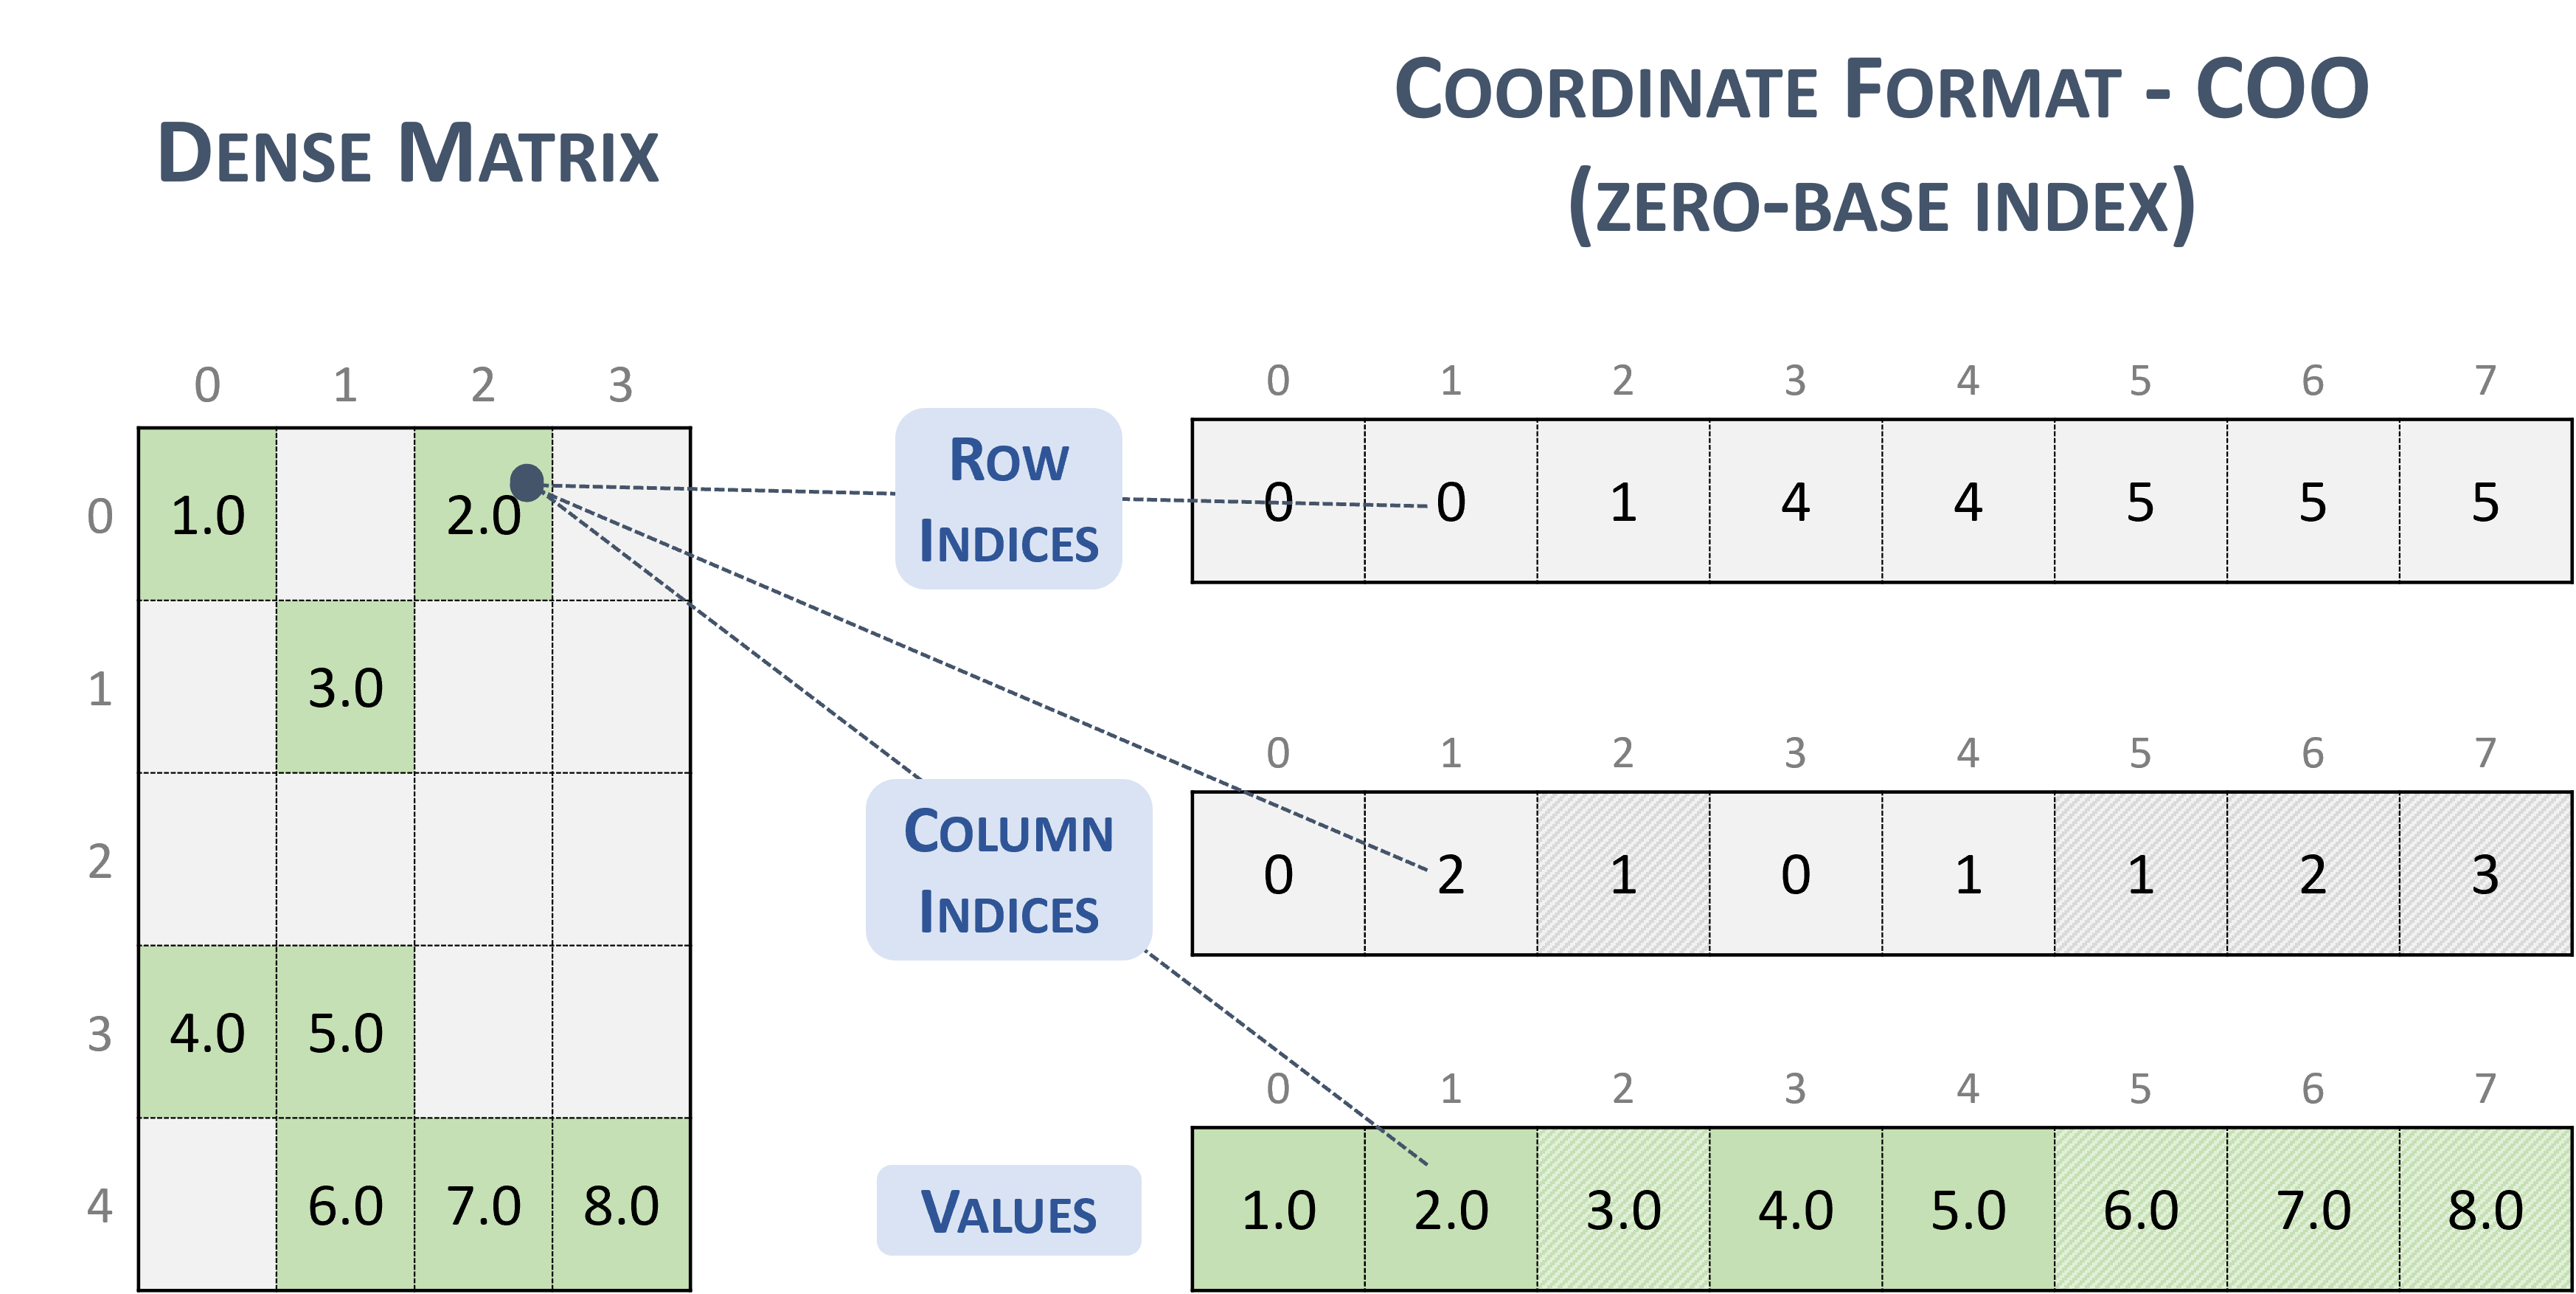
\includegraphics[width=\textwidth]{img/coo.png}
		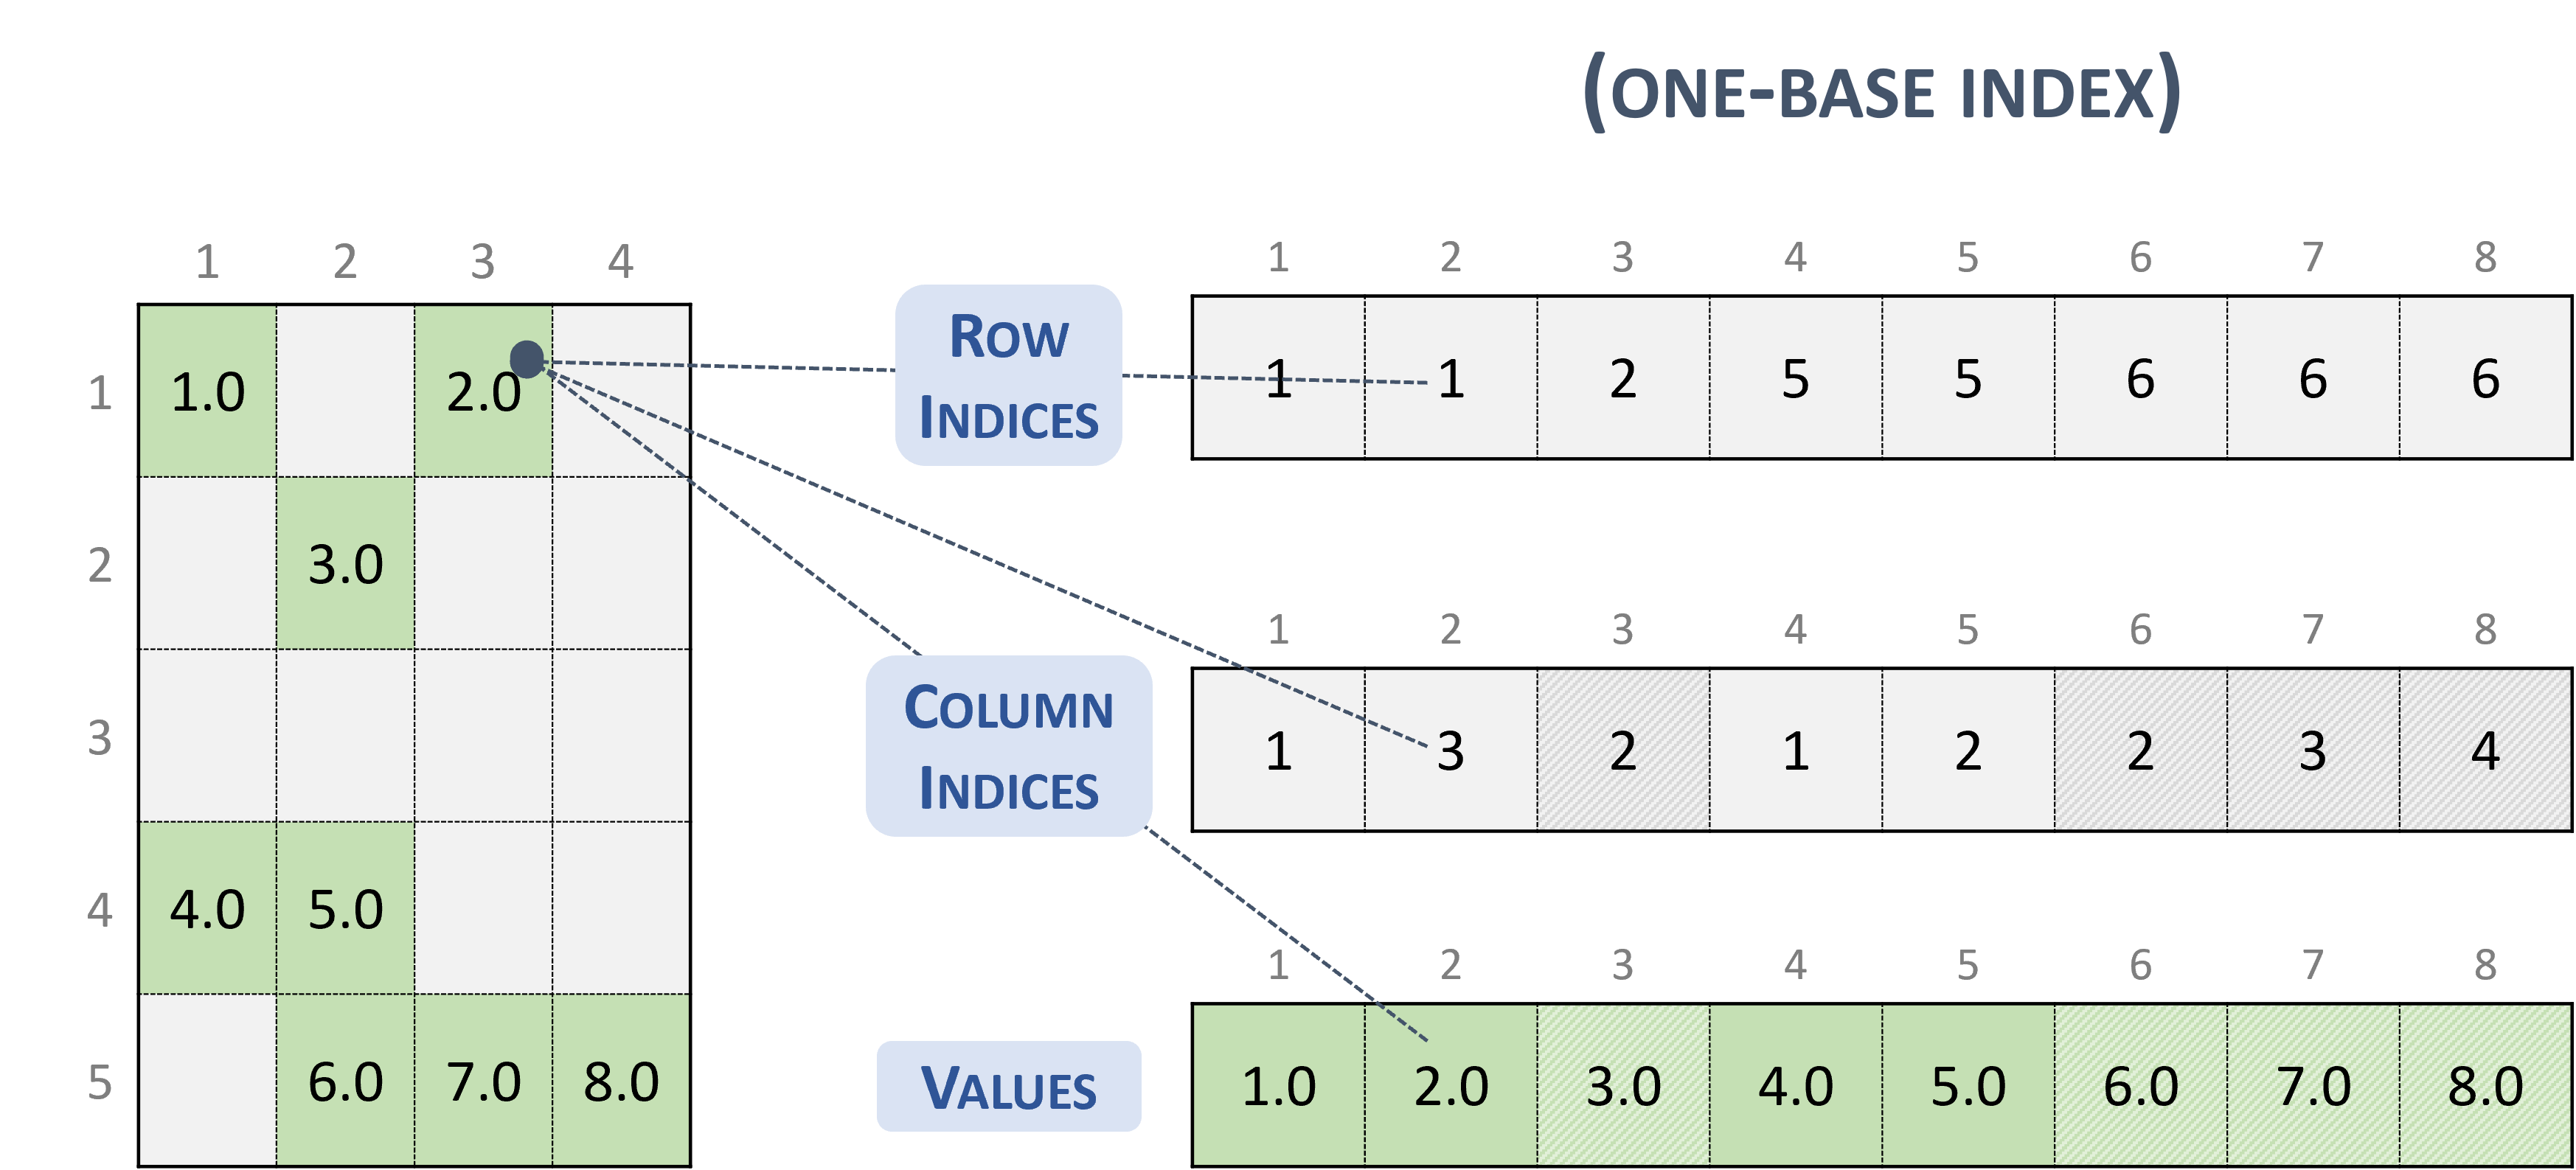
\includegraphics[width=\textwidth]{img/coo_one_base.png}
		\caption{Graphical representation of the coordinate format (COO) technique. From the figure we can see the representation of the \texttt{AA} array, called \emph{values}, the \texttt{JR}, called \emph{row indices}, and finally the \texttt{JC}, called \emph{column indices}. The algorithm is very simple. The figures are taken from the \href{https://docs.nvidia.com/nvpl/_static/sparse/storage_format/sparse_matrix.html}{NVIDIA Performance Libraries Sparse}, which is part of the \href{https://developer.nvidia.com/nvpl}{NVIDIA Performance Libraries}.}
	\end{figure}
	
	\item \definition{Coordinate Compressed Sparse Row format (CSR)}. If the elements of $A$ are listed by row, the array \texttt{JC} might be replaced by an array that points to the beginning of each row.
	\begin{itemize}
		\item \texttt{AA}: all the values of the non-zero elements of $A$, stored row by row from $1, \dots, n$.
		
		\item \texttt{JA}: contains the column indices.
		
		\item \texttt{IA}: contains the pointers to the beginning of each row in the arrays $A$ and \texttt{JA}. Thus \texttt{IA}$\left(i\right)$ contains the position in the arrays \texttt{AA} and \texttt{JA} where the $i$-th row starts. The length of \texttt{IA} is $n+1$, with $\texttt{IA}\left(n+1\right)$ containing the number $A\left(1\right) + \nnz\left(A\right)$. Remember that $n$ is the number of rows.
	\end{itemize}
	For \example{example}:
	\begin{equation*}
		A = \begin{bmatrix}
			1. & 0. & 0.& 2. & 0. \\
			3. & 4. & 0.& 5. & 0. \\
			6. & 0. & 7.& 8. & 9. \\
			0. & 0. & 10.& 11. & 0. \\
			0. & 0. & 0.& 0. & 12. 
		\end{bmatrix}
	\end{equation*}
	\begin{equation*}
		\begin{array}{rcl}
			\texttt{AA} &=& \left[
				1.\hspace{1em}
				2.\hspace{1em}
				3.\hspace{1em}
				\phantom{1}4.\hspace{1em}
				\phantom{1}5.\hspace{1em}
				\phantom{1}6.\hspace{1em}
				7.\hspace{1em}
				8.\hspace{1em}
				9.\hspace{1em}
				10.\hspace{1em}
				11.\hspace{1em}
				12.
			\right] \\ [.5em]
			\texttt{JA} &=& \left[
				1\phantom{.}\hspace{1em}
				4\phantom{.}\hspace{1em}
				1\phantom{.}\hspace{1em}
				\phantom{1}2\phantom{.}\hspace{1em}
				\phantom{1}4\phantom{.}\hspace{1em}
				\phantom{1}1\phantom{.}\hspace{1em}
				3\phantom{.}\hspace{1em}
				4\phantom{.}\hspace{1em}
				5\phantom{.}\hspace{1em}
				\phantom{1}3\phantom{.}\hspace{1em}
				\phantom{1}4\phantom{.}\hspace{1em}
				\phantom{1}5\phantom{.}
			\right] \\ [.5em]
			\texttt{IA} &=& \left[
				1\phantom{.}\hspace{1em}
				3\phantom{.}\hspace{1em}
				6\phantom{.}\hspace{1em}
				10\phantom{.}\hspace{1em}
				12\phantom{.}\hspace{1em}
				13\phantom{.}
			\right]
		\end{array}
	\end{equation*}
	To retrieve each position of the matrix, the algorithm is quite simple. Consider the \texttt{IA} arrays. 
	\begin{enumerate}
		\item We start at position one of the array, then the value 1:
		\begin{equation*}
			\begin{array}{rcl}
				\texttt{AA} &=& \left[
				1.\hspace{1em}
				2.\hspace{1em}
				3.\hspace{1em}
				\phantom{1}4.\hspace{1em}
				\phantom{1}5.\hspace{1em}
				\phantom{1}6.\hspace{1em}
				7.\hspace{1em}
				8.\hspace{1em}
				9.\hspace{1em}
				10.\hspace{1em}
				11.\hspace{1em}
				12.
				\right] \\ [.5em]
				\texttt{JA} &=& \left[
				1\phantom{.}\hspace{1em}
				4\phantom{.}\hspace{1em}
				1\phantom{.}\hspace{1em}
				\phantom{1}2\phantom{.}\hspace{1em}
				\phantom{1}4\phantom{.}\hspace{1em}
				\phantom{1}1\phantom{.}\hspace{1em}
				3\phantom{.}\hspace{1em}
				4\phantom{.}\hspace{1em}
				5\phantom{.}\hspace{1em}
				\phantom{1}3\phantom{.}\hspace{1em}
				\phantom{1}4\phantom{.}\hspace{1em}
				\phantom{1}5\phantom{.}
				\right] \\ [.5em]
				\texttt{IA} &=& \left[
				\circledtext{1}\phantom{.}\hspace{.4em}
				3\phantom{.}\hspace{1em}
				6\phantom{.}\hspace{1em}
				10\phantom{.}\hspace{1em}
				12\phantom{.}\hspace{1em}
				13\phantom{.}
				\right]
			\end{array}
		\end{equation*}
		
		
		\item We use the value one to see the first (index one) position of the array JA, and the value is 1:
		\begin{equation*}
			\begin{array}{rcl}
				\texttt{AA} &=& \left[
				1.\hspace{1em}
				2.\hspace{1em}
				3.\hspace{1em}
				\phantom{1}4.\hspace{1em}
				\phantom{1}5.\hspace{1em}
				\phantom{1}6.\hspace{1em}
				7.\hspace{1em}
				8.\hspace{1em}
				9.\hspace{1em}
				10.\hspace{1em}
				11.\hspace{1em}
				12.
				\right] \\ [.5em]
				\texttt{JA} &=& \left[
				\circledtext{1}\phantom{.}\hspace{.4em}
				4\phantom{.}\hspace{1em}
				1\phantom{.}\hspace{1em}
				\phantom{1}2\phantom{.}\hspace{1em}
				\phantom{1}4\phantom{.}\hspace{1em}
				\phantom{1}1\phantom{.}\hspace{1em}
				3\phantom{.}\hspace{1em}
				4\phantom{.}\hspace{1em}
				5\phantom{.}\hspace{1em}
				\phantom{1}3\phantom{.}\hspace{1em}
				\phantom{1}4\phantom{.}\hspace{1em}
				\phantom{1}5\phantom{.}
				\right] \\ [.5em]
				\texttt{IA} &=& \left[
				1\phantom{.}\hspace{1em}
				3\phantom{.}\hspace{1em}
				6\phantom{.}\hspace{1em}
				10\phantom{.}\hspace{1em}
				12\phantom{.}\hspace{1em}
				13\phantom{.}
				\right]
			\end{array}
		\end{equation*}
		
		\item But with the same index of \texttt{IA}, you also check the array \texttt{AA}, which has a value of 1:
		\begin{equation*}
			\begin{array}{rcl}
				\texttt{AA} &=& \left[
				\circledtext{1.}\hspace{.6em}
				2.\hspace{1em}
				3.\hspace{1em}
				\phantom{1}4.\hspace{1em}
				\phantom{1}5.\hspace{1em}
				\phantom{1}6.\hspace{1em}
				7.\hspace{1em}
				8.\hspace{1em}
				9.\hspace{1em}
				10.\hspace{1em}
				11.\hspace{1em}
				12.
				\right] \\ [.5em]
				\texttt{JA} &=& \left[
				1\phantom{.}\hspace{1em}
				4\phantom{.}\hspace{1em}
				1\phantom{.}\hspace{1em}
				\phantom{1}2\phantom{.}\hspace{1em}
				\phantom{1}4\phantom{.}\hspace{1em}
				\phantom{1}1\phantom{.}\hspace{1em}
				3\phantom{.}\hspace{1em}
				4\phantom{.}\hspace{1em}
				5\phantom{.}\hspace{1em}
				\phantom{1}3\phantom{.}\hspace{1em}
				\phantom{1}4\phantom{.}\hspace{1em}
				\phantom{1}5\phantom{.}
				\right] \\ [.5em]
				\texttt{IA} &=& \left[
				1\phantom{.}\hspace{1em}
				3\phantom{.}\hspace{1em}
				6\phantom{.}\hspace{1em}
				10\phantom{.}\hspace{1em}
				12\phantom{.}\hspace{1em}
				13\phantom{.}
				\right]
			\end{array}
		\end{equation*}
		
		\item Now we can check the next row of the matrix. So we check the array \texttt{IA} at position 2 and get the value 3. But be careful! From 1 (the previously calculated value) to 3 (the value just taken) there is the value 2 in between. So we can assume that the value 2 is also in the first row.
		\begin{equation*}
			\begin{array}{rcl}
				\texttt{AA} &=& \left[
				1.\hspace{1em}
				\circledtext{2.}\hspace{.6em}
				3.\hspace{1em}
				\phantom{1}4.\hspace{1em}
				\phantom{1}5.\hspace{1em}
				\phantom{1}6.\hspace{1em}
				7.\hspace{1em}
				8.\hspace{1em}
				9.\hspace{1em}
				10.\hspace{1em}
				11.\hspace{1em}
				12.
				\right] \\ [.5em]
				\texttt{JA} &=& \left[
				1\phantom{.}\hspace{1em}
				\circledtext{4}\phantom{.}\hspace{.4em}
				1\phantom{.}\hspace{1em}
				\phantom{1}2\phantom{.}\hspace{1em}
				\phantom{1}4\phantom{.}\hspace{1em}
				\phantom{1}1\phantom{.}\hspace{1em}
				3\phantom{.}\hspace{1em}
				4\phantom{.}\hspace{1em}
				5\phantom{.}\hspace{1em}
				\phantom{1}3\phantom{.}\hspace{1em}
				\phantom{1}4\phantom{.}\hspace{1em}
				\phantom{1}5\phantom{.}
				\right] \\ [.5em]
				\texttt{IA} &=& \left[
				1\phantom{.}\hspace{1.3em}
				3\phantom{.}\hspace{.7em}
				6\phantom{.}\hspace{1em}
				10\phantom{.}\hspace{1em}
				12\phantom{.}\hspace{1em}
				13\phantom{.}
				\right]
			\end{array}
		\end{equation*}
	\end{enumerate}
	\newpage
	\begin{figure}[!htp]
		\centering
		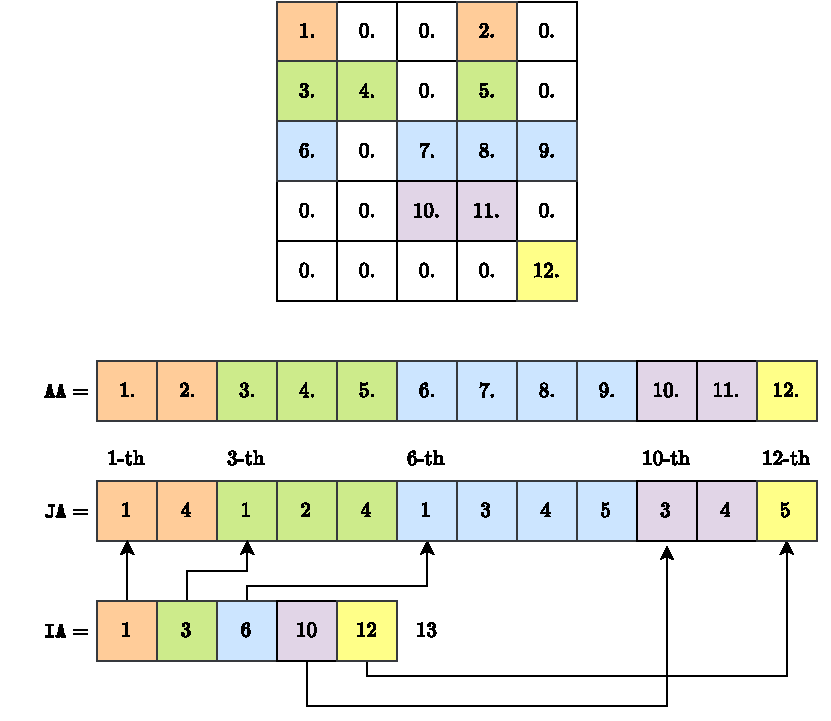
\includegraphics[width=\textwidth]{img/crs.pdf}
		\caption{View an illustration of the CRS technique using colors to improve readability.}
	\end{figure}
	\begin{figure}[!htp]
		\centering
		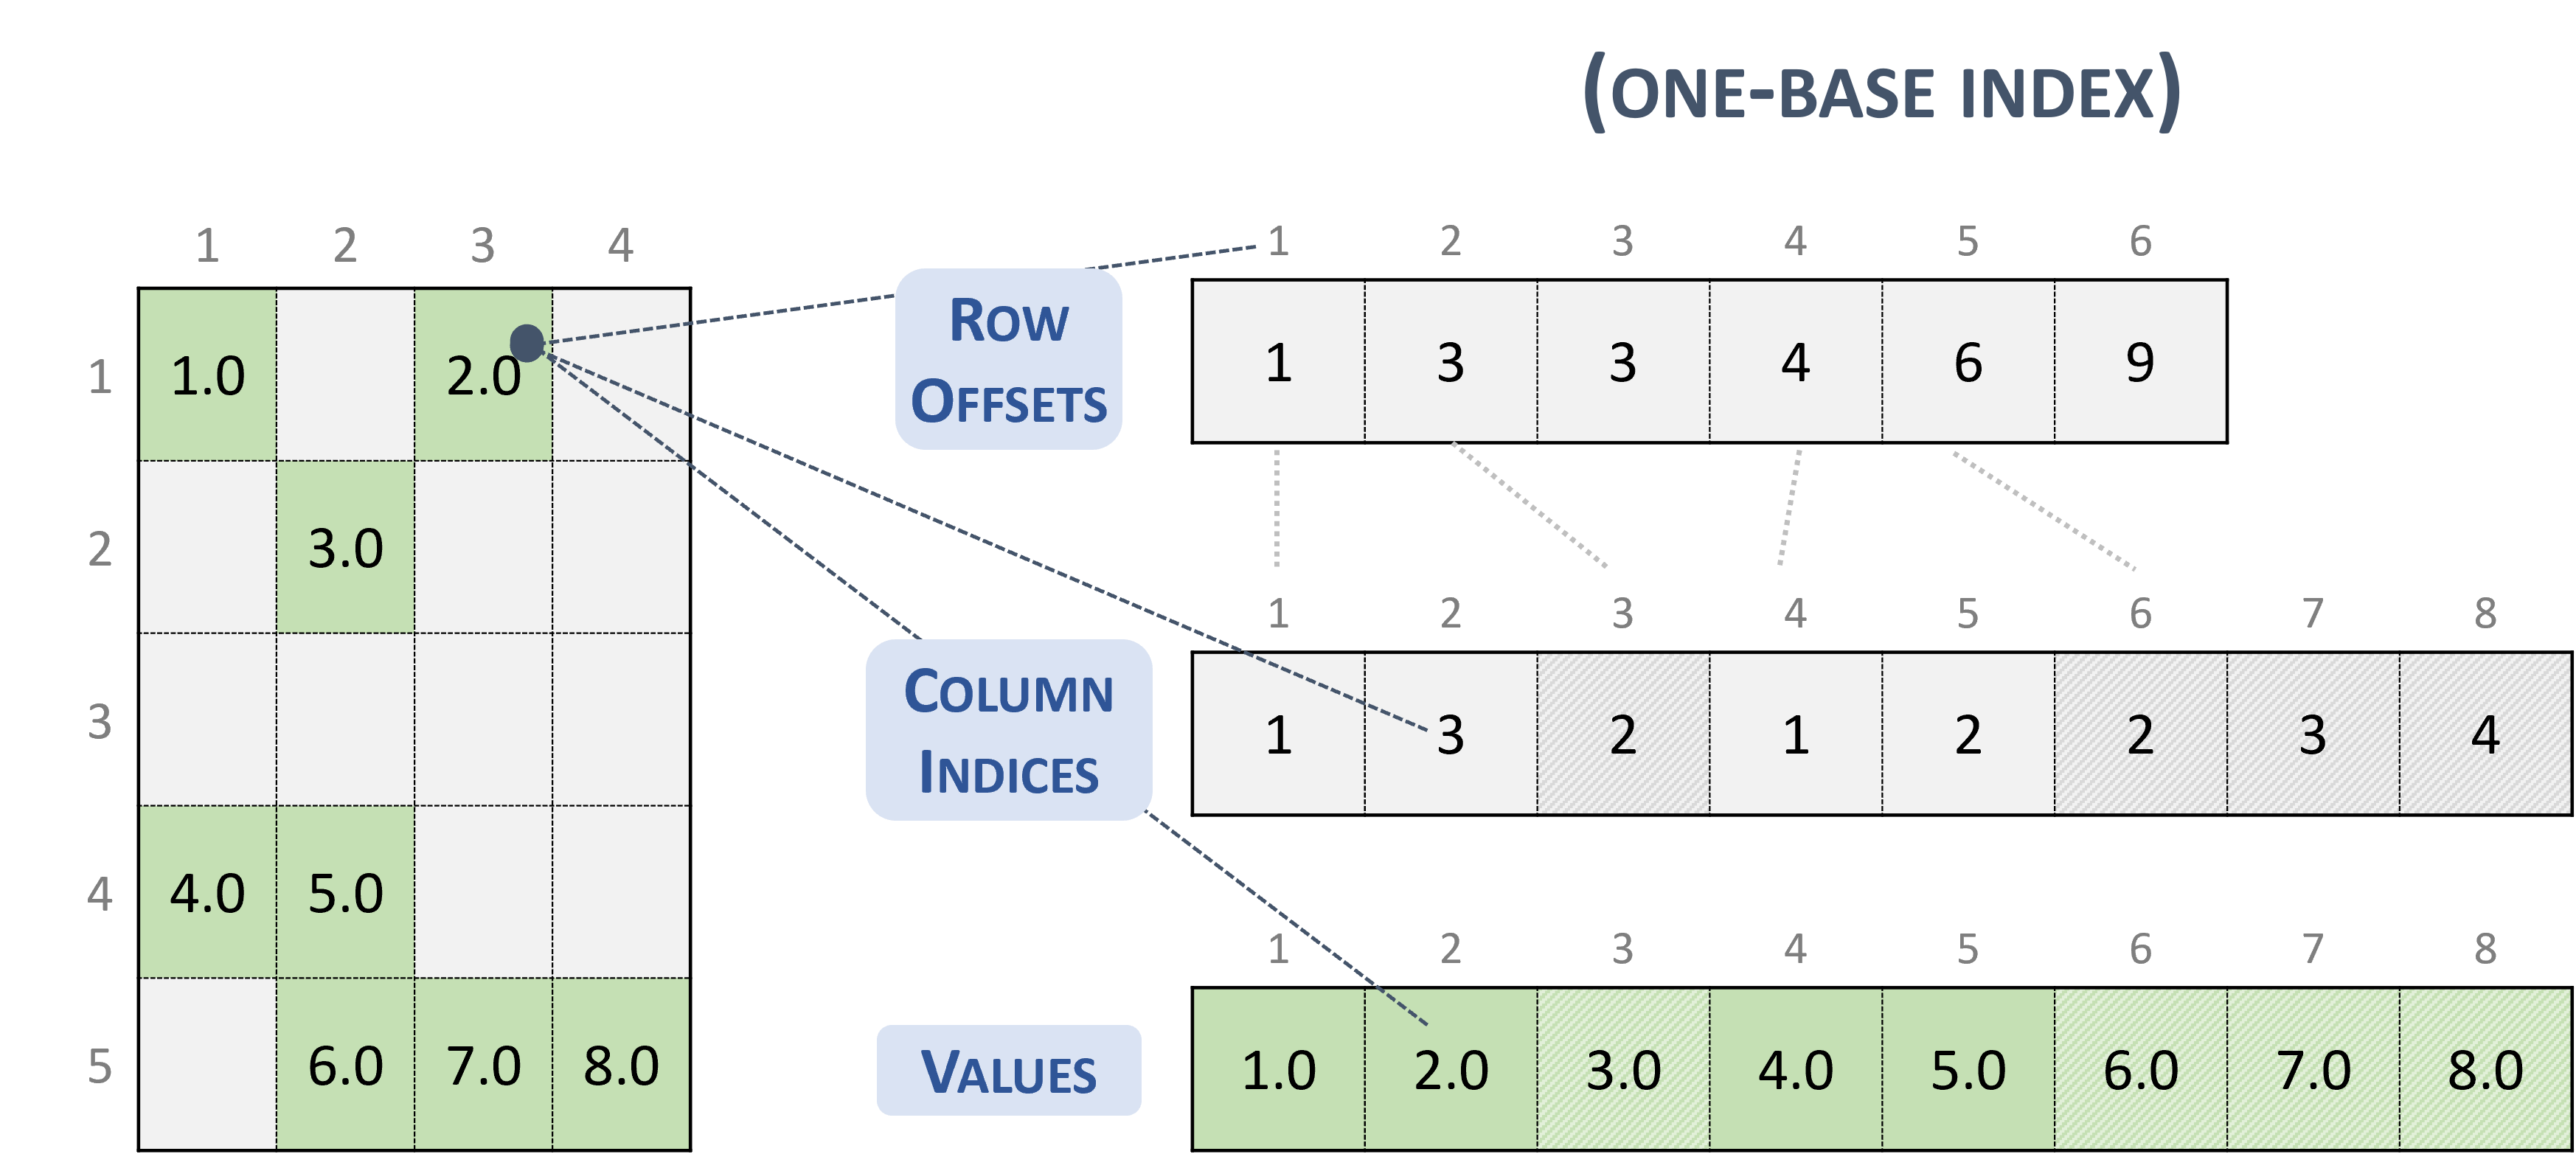
\includegraphics[width=.9\textwidth]{img/csr_one_base.png}
		\caption{Graphical representation of the coordinate compressed sparse row (CSR) technique. From the figure we can see the representation of the \texttt{AA} array, called \emph{values}, the \texttt{IA}, called \emph{row offset}, and finally the \texttt{JA}, called \emph{column indices}.
		It's interesting to see how the empty line case is handled. It copies the previous value of the array.
		The figures are taken from the \href{https://docs.nvidia.com/nvpl/_static/sparse/storage_format/sparse_matrix.html}{NVIDIA Performance Libraries Sparse}, which is part of the \href{https://developer.nvidia.com/nvpl}{NVIDIA Performance Libraries}.}
	\end{figure}
\end{itemize}

    %%%%%%%%%%%%%%%%%%%%%%%%%%%%%%%%%%%%%%%%%%%%%%%%%%%%%
    % Iterative methods for linear systems of equations %
    %%%%%%%%%%%%%%%%%%%%%%%%%%%%%%%%%%%%%%%%%%%%%%%%%%%%%
    \section{Iterative methods for linear systems of equations}

\subsection{Why not use the direct methods?}

Let us considering the following linear system of equations:
\begin{equation*}
    Ax = b
\end{equation*}
Where $A \in \mathbb{R}^{n \times n}$, $b \in \mathbb{R}^{n}$, $x \in \mathbb{R}^{n}$ and $\det\left(A\right) \ne 0$. In general, direct methods are \textbf{not very suitable whenever}:
\begin{itemize}
    \item \textbf{$n$ is large}. Typically, the average cost of direct methods scales as $n^{3}$, except in selected cases. As a trivial example, if peak performance is 1 PetaFLOPS ($10^{15}$ floating point operations per second), then
    \begin{equation*}
        n = 10^{7} \rightarrow \approx 10^{6} \text{ seconds} \approx 11 \text{ days}
    \end{equation*}
    \item \textbf{Matrix $A$ is sparse}. Direct methods suffer from the \emph{fill-in} phenomenon\footnote{The fill-in of a matrix are those entries that change from an initial zero to a non-zero value during the execution of an algorithm. To reduce the memory requirements and the number of arithmetic operations used during an algorithm, it is useful to minimize the fill-in.} (see later). Unfortunately, sparse matrices are very popular in many application problems and we cannot consider them.
\end{itemize}

\highspace
\begin{definitionbox}[: Sparse Matrix]
    Let $A \in \mathbb{R}^{n \times n}$ we say that $A$ is \definitionWithSpecificIndex{sparse}{Sparse Matrix} the number of non-zero elements (abbreviated as $\nnz\left(A\right)$) is approximately equal to the number of rows/columns $n$, i.e. $\nnz\left(A\right) \sim n$.
\end{definitionbox}

\highspace
\begin{flushleft}
    \textcolor{Green3}{\faIcon{question-circle} \textbf{What is an iterative method?}}
\end{flushleft}
It is clear that iterative methods are usually better than direct methods. An \definitionWithSpecificIndex{iterative method}{Iterative Method} is a \textbf{mathematical procedure that uses an initial value to generate a sequence of improving approximate solutions to a class of problems}, where the $i$-th approximation (called an \dquotes{\emph{iteration}}) is derived from the previous ones.

\highspace
More precisely, we introduce a sequence $\mathbf{x}^{\left(k\right)}$ of vectors determined by a recursive relation that identifies the method.
\begin{equation*}
    \mathbf{x}^{\left(0\right)} \rightarrow
    \mathbf{x}^{\left(1\right)} \rightarrow
    \cdots \rightarrow
    \mathbf{x}^{\left(k\right)} \rightarrow
    \mathbf{x}^{\left(k+1\right)} \rightarrow
    \cdots
\end{equation*}
To \dquotes{\emph{initialize}} the iterative process, it is necessary to provide a starting point (\emph{initial vector}, also called \emph{initial guess}) $\mathbf{x}^{\left(0\right)}$, e.g. based on physical/engineering applications.

\newpage

\noindent
After initialization, the core of the process should, sooner or later, produce a result. It is a very complex and long topic, but in general it refers to the process by which an iterative algorithm approaches a fixed point or a solution to a problem after several iterations. An \textbf{iterative method must satisfy the} \definitionWithSpecificIndex{convergence property}{Convergence property}:
\begin{equation}\label{eq: convergence property}
    \lim\limits_{k \rightarrow + \infty} \mathbf{x}^{\left(k\right)} = \mathbf{x}
\end{equation}
It is important to note that the \textbf{convergence \underline{does not depend} on the choice of the initial vector} $x^{\left(0\right)}$.

\highspace
From the property \ref{eq: convergence property}, it should be clear that \textbf{convergence is guaranteed only after an $\infty$ number of iterations}. From a practical point of view, we need to stop the iteration process after a finite number of iterations when we are \emph{sufficiently close} to the solution.

\highspace
In addition to the \emph{problem of convergence} and \dquotes{\emph{when should we stop our convergence method}}, we have to deal with the \emph{numerical error} inevitably introduced by our method.

\highspace
These topics will be explained and faced in the following pages.
    \subsection{Linear iterative methods}

\subsubsection{Definition}

In general, we consider linear iterative methods of the following form:
\begin{equation*}
    \mathbf{x}^{\left(k+1\right)} = B\mathbf{x}^{\left(k\right)} + \mathbf{f} \hspace{2em} k \ge 0
\end{equation*}
Where $B \in \mathbb{R}^{n \times n}$, $\mathbf{f} \in \mathbb{R}^{n}$ and the matrix $B$ is called \textbf{iteration matrix}. The choice of the iteration matrix and $\mathbf{f}$ uniquely identifies the method.

\highspace
The question is now automatic. \textbf{How to choose} an intelligent iteration matrix and $\mathbf{f}$? There are two main factors to consider:
\begin{itemize}
    \item \textbf{\underline{Consistency}}. This is a necessary condition, but not sufficient to guarantee the convergence. If $\mathbf{x}^{\left(k\right)}$ es the exact solution $\mathbf{x}$, then $\mathbf{x}^{\left(k+1\right)}$ is again equal to $\mathbf{x}$ (no update if the exact solution is found):
    \begin{equation*}
        \mathbf{x} = B \mathbf{x} + \mathbf{f} \longrightarrow \mathbf{f} = \left(I-B\right)\mathbf{x} = \left(I-B\right)A^{-1}\mathbf{b}
    \end{equation*}
    The former identity gives a relationship between $B$ and $\mathbf{f}$ as a function of the data.

    \item \textbf{\underline{Convergence}}. To study the convergence we need the error and the spectral radius:
    \begin{itemize}
        \item \textbf{Error}. Let us introduce the error at step $\left(k+1\right)$:
        \begin{equation*}
            \mathbf{e}^{\left(k+1\right)} = \mathbf{x} - \mathbf{x}^{\left(k+1\right)}
        \end{equation*}
        And an appropriate vector norm, such as the Euclidean norm $\vectorNormSymbol$.
        
        Then we have:
        \begin{equation*}
            \begin{array}{rcl}
                \left|\left|\mathbf{e}^{\left(k+1\right)}\right|\right| &=& \left|\left|\mathbf{x}-\mathbf{x}^{\left(k+1\right)}\right|\right| \\ [.5em]
                %
                &=& \left|\left|\mathbf{x}-\left(B\mathbf{x}^{\left(k\right)} + \mathbf{f}\right)\right|\right| \\ [.5em]
                %
                &=& \left|\left|\mathbf{x}-B\mathbf{x}^{\left(k\right)} - \mathbf{f}\right|\right| \\ [.5em]
                %
                &=& \left|\left|\mathbf{x}-B\mathbf{x}^{\left(k\right)} - \left(I-B\right)\mathbf{x}\right|\right| \\ [.5em]
                %
                &=& \left|\left|\mathbf{x}-B\mathbf{x}^{\left(k\right)} - I\mathbf{x} + B\mathbf{x}\right|\right| \\ [.5em]
                %
                &=& \left|\left|\mathbf{x}-B\mathbf{x}^{\left(k\right)} - \mathbf{x} + B\mathbf{x}\right|\right| \\ [.5em]
                %
                &=& \left|\left|-B\mathbf{x}^{\left(k\right)} + B\mathbf{x}\right|\right| \\ [.5em]
                %
                &=& \left|\left|B\left(\mathbf{x} - \mathbf{x}^{\left(k\right)}\right)\right|\right| \\ [.5em]
                %
                &=& \left|\left|B\mathbf{e}^{\left(k\right)}\right|\right| \\ [.5em]
                %
                &\le& \left|\left|B\right|\right| \cdot \left|\left|\mathbf{e}^{\left(k\right)}\right|\right|
            \end{array}
        \end{equation*}
        Note that $\left|\left|B\right|\right|$ is the matrix norm induced by the vector norm $\vectorNormSymbol$.

        Using recursion, we get:
        \begin{equation*}
            \begin{array}{rcl}
                \left|\left|\mathbf{e}^{\left(k+1\right)}\right|\right| &\le& \left|\left|B\right|\right| \cdot \left|\left|\mathbf{e}^{\left(k\right)}\right|\right| \\ [.5em]
                %
                &\le& \left|\left|B\right|\right| \cdot \left|\left|B\right|\right| \cdot \left|\left|\mathbf{e}^{\left(k-1\right)}\right|\right| \\ [.5em]
                %
                &\le& \left|\left|B\right|\right| \cdot \left|\left|B\right|\right| \cdot \left|\left|B\right|\right| \cdot \left|\left|\mathbf{e}^{\left(k-2\right)}\right|\right| \\ [.5em]
                %
                &\le& \cdots \\ [.5em]
                %
                &\le& {\left|\left|B\right|\right|}^{\left(k+1\right)} \cdot \left|\left|\mathbf{e}^{\left(0\right)}\right|\right| \\ [.5em]
                %
                \lim\limits_{k \rightarrow \infty} \left|\left|\mathbf{e}^{\left(k+1\right)}\right|\right| &\le& \left(\lim\limits_{k \rightarrow \infty} {\left|\left|B\right|\right|}^{\left(k+1\right)}\right) \cdot \left|\left|\mathbf{e}^{\left(0\right)}\right|\right|
            \end{array}
        \end{equation*}
        And here is the key. The \textbf{sufficient condition for convergence is to choose a matrix $B$ that has the norm less than $1$}:
        \begin{equation*}
            \left|\left|B\right|\right| < 1 \Longrightarrow \lim\limits_{k \rightarrow \infty} \left|\left|\mathbf{e}^{\left(k+1\right)}\right|\right| = 0
        \end{equation*}
        We recall that the \emph{Euclidean norm} (commonly used) of a matrix is calculated by taking the square root of the sum of the absolute squares of its elements. Let $A$ be a matrix of size $m \times n$, the Euclidean norm:
        \begin{equation*}
            {\left|\left|A\right|\right|}_{2} \equiv \sqrt{\displaystyle\sum_{i=1}^{m}\sum_{j=1}^{n} {\left|a_{ij}\right|}^{2}}
        \end{equation*}
        
        
        \item \textbf{Spectral radius}. The spectral radius of a matrix is the \textbf{largest absolute value of its eigenvalues}. We define:
        \begin{equation*}
            \rho\left(B\right) = \underset{j}{\max} \left|\lambda_{j}\left(B\right)\right|
        \end{equation*}
        Where $\lambda_{j}\left(B\right)$ are the eigenvalues of $B$.

        Why is the spectral radius useful? Well, if the matrix $B$ is symmetric positive definite (SPD)\footnote{\definition{SPD (Symmetric Positive Definite)} is a matrix: \begin{itemize}
            \item Symmetric: $A = A^{T}$
            \item Positive Definite: $x^{T}AX > 0$, $\forall x \in \mathbb{R}^{n} \setminus \left\{0\right\}$
        \end{itemize}}, then the spectral radius is equal to the Euclidean norm of the matrix.
        \begin{equation*}
            B \text{ is SPD } \Rightarrow {\left|\left|B\right|\right|}_{2} = \rho\left(B\right) \: \land \: \rho\left(B\right) < 1 \iff \text{method convergences}
        \end{equation*}
        And this is a very big help to us for many reasons.
        \begin{itemize}
            \item \textbf{Balance and Predictability}. When the norm is equal to the spectral, it means that the influence of the matrix is well distributed. In other words, this uniformity can help make our iterative methods more predictable, reducing the possibility of non-convergence.

            \item \textbf{Efficiency}. It avoids scenarios where the matrix might have hidden large entries affecting convergence or stability.
        \end{itemize}   
    \end{itemize}
\end{itemize}
\newpage
\noindent
Let $C \in \mathbb{R}^{n \times n}$ then the spectral radius of a matrix is equal to the \href{https://en.wikipedia.org/wiki/Infimum_and_supremum}{infimum} (lower bound) of its matrix norm:
\begin{equation}
    \rho\left(C\right) = \mathrm{inf}\left\{ \left|\left|C\right|\right| \:\: \forall \text{ induced matrix norm }\vectorNormSymbol\right\}
\end{equation}
It follows from this property that:
\begin{equation}\label{eq: spectral radius less/equal than norm}
    \rho\left(B\right) \le \left|\left|B\right|\right| \hspace{2em} \forall \text{induced matrix norm } \vectorNormSymbol
\end{equation}
Note that thanks to \ref{eq: spectral radius less/equal than norm} we can observe that if:
\begin{equation*}
    \exists \vectorNormSymbol \: \text{such that} \: \left|\left|B\right|\right| < 1 \Longrightarrow \rho\left(B\right) < 1
\end{equation*}
The convergence of the method is guaranteed by the following theorem.

\highspace
\begin{theorem}[\textbf{necessary and sufficient condition for convergence}]
    A \textbf{consistent} iterative method with iteration matrix B converges if and only if $\rho\left(B\right) < 1$.
\end{theorem}

\newpage

\subsubsection{Jacobi method}

Let the problem of solve $Ax = b$, where $A$ is a square matrix, $x$ is the vector of unknowns, and $b$ is the result vector.

\highspace
We start from the $i$-th line of the linear system:
\begin{equation*}
    \displaystyle\sum_{j = 1}^{n} a_{ij}x_{j} = b_{i} \: \rightarrow \: a_{i1}x_{1} + a_{i2}x_{2} + \cdots + a_{in}x_{n} = b_{i}
\end{equation*}
Formally the solution $x_{i}$ for each $i$ si given by:
\begin{equation}
    x_{i} = \dfrac{b_{i}-\displaystyle\sum_{j \ne i} a_{ij}x_{j}}{a_{ii}}
\end{equation}
Obviously the previous identity cannot be used in practice because we do not know $x_{j}$, for $j \ne i$. And here is the \textbf{magic idea} of Jacobi: we could think of introducing an iterative method (Jacobi) that \textbf{updates} $x_{i}^{\left(k+1\right)}$ \textbf{step} $k+1$ \textbf{using the other} $x_{j}^{\left(k\right)}$ \textbf{obtained in the previous step} $k$.
\begin{equation}\label{eq: jacobi x calcolus}
    x_{i} = \dfrac{b_{i}-\displaystyle\sum_{j \ne i} a_{ij}x_{j}}{a_{ii}} \: \xRightarrow{\text{as }x_{j}\text{ is not well known}} \: x_{i}^{\left(k+1\right)} = \dfrac{b_{i}-\displaystyle\sum_{j \ne i} a_{ij}x_{j}^{\left(k\right)}}{a_{ii}}
\end{equation}
Where $\forall i = 1, \dots, n$.

\highspace
\begin{flushleft}
    \textcolor{Green3}{\faIcon{tools} \textbf{Algorithm}}
\end{flushleft}
\begin{enumerate}
    \item \textbf{Start with an initial guess} $x^{\left(0\right)}$, also zero.
    \item \textbf{Update each component} $x_{i}^{\left(k+1\right)}$ using the equation \ref{eq: jacobi x calcolus}.
    \item \textbf{Repeat until the changes are less than a specified tolerance} or we haven't found the exact solution (in practice very difficult, almost impossible).
\end{enumerate}

\highspace
\begin{flushleft}
    \textcolor{Red2}{\faIcon{dollar-sign} \textbf{How much does it cost?}}
    \label{general-ref: cost jacobi method}
\end{flushleft}
It depends on the matrix used:
\begin{itemize}
    \item \textbf{Dense matrix} (bad choice). Each iteration costs $\approx n^{2}$ operations, so the Jacobi method is competitive if the number of iteration is less than $n$.
    \item \textbf{Sparse matrix} (good choice). Each iteration costs only $\approx n$ operations.
\end{itemize}

\highspace
\begin{flushleft}
    \textcolor{Green3}{\faIcon{network-wired} \textbf{Can it be parallelized?}}
\end{flushleft}
The parallelization of the Jacobi method is actually \textbf{one of its main advantages} on modern computers. Each update of $x_{i}$ depends only on the previous values of the other $x_{j}$, not on the current iteration values. This independence makes it easy to distribute the work across multiple processors.

\newpage

\subsubsection{Gauss-Seidel method}

Given the Jacobi method, the Gauss Seidel method is similar, but with one clever difference: it uses the latest available values during iterations.
\begin{equation}\label{eq: gauss seidel x calcolus}
    x_{i}^{\left(k+1\right)} = \dfrac{b_{i} - \displaystyle\sum_{j < i} a_{ij}x_{j}^{\left(k+1\right)} - \displaystyle\sum_{j > i}a_{ij}x_{j}^{\left(k\right)}}{a_{ii}}
\end{equation}
At iteration $\left(k+1\right)$, let's consider the computation of $x_{i}^{\left(k+1\right)}$. we observer that for $j < i$ (with $i \ge 2$), $x_{j}^{\left(k+1\right)}$ is known (we have already calculated it). We can therefore think of using the quantities at step $\left(k+1\right)$ if $j<i$ and, as in the Jacobi method, those at the previous step $k$ if $j > i$.

\highspace
\begin{flushleft}
    \textcolor{Green3}{\faIcon{tools} \textbf{Algorithm}}
\end{flushleft}
\begin{enumerate}
    \item \textbf{Start with an initial guess} $x^{\left(0\right)}$, also zero.
    \item \textbf{Iteration}. For each row $i$ from $1$ to $n$ calculate the value of the equation \ref{eq: gauss seidel x calcolus}.
    \item \textbf{Repeat until the changes are less than a specified tolerance}.
\end{enumerate}

\highspace
\begin{flushleft}
    \textcolor{Red2}{\faIcon{dollar-sign} \textbf{How much does it cost?}}
\end{flushleft}
The cost is comparable to the Jacobi method explained on page \pageref{general-ref: cost jacobi method}.

\highspace
\begin{flushleft}
    \textcolor{Green3}{\faIcon{network-wired} \textbf{Can it be parallelized?}}
\end{flushleft}
Unlike the Jacobi method, the Gauss-Seidel method relies on the most recent updates within the same iteration. This sequential dependency \textbf{makes it more difficult to parallelize, as each update depends on the previous ones}.

\highspace
While it's harder to parallelize due to its inherent sequential nature, we can still achieve some degree of parallelism with clever strategies such as red-black ordering. This makes the Gauss-Seidel method less straightforward to parallelize than Jacobi, but not impossible.

\newpage

\subsubsection{Convergence of Jacobi and Gauss-Seidel methods}

Let be a general matrix $A$, and :
\begin{itemize}
    \item $D$ the \textbf{diagonal part} of $A$
    \item $-E$ \textbf{lower triangular part} of $A$
    \item $-F$ \textbf{upper triangular part} of $A$
\end{itemize}
\begin{equation*}
    A = \begin{bmatrix}
        & & & & \\
        & \ddots &   & -F     & \\
        &        & D &        & \\
        & -E     &   & \ddots & \\
        & & & &
    \end{bmatrix}
\end{equation*}
The previous Jacobi and Gauss-Seidel methods can be rewritten as:
\begin{itemize}
    \item Jacobi:
    \begin{itemize}
        \item Method:
        \begin{equation*}
            D\mathbf{x}^{\left(k+1\right)} = \left(E+F\right)\mathbf{x}^{\left(k\right)} + \mathbf{b}
        \end{equation*}
        \item Iteration matrix:
        \begin{equation*}
            B_{J} = D^{-1}\left(E+F\right) = D^{-1}\left(D-A\right) = I-D^{-1}A
        \end{equation*}
    \end{itemize}

    \item Gauss-Seidel
    \begin{itemize}
        \item Method:
        \begin{equation*}
            \left(D-E\right)\mathbf{x}^{\left(k+1\right)} = F\mathbf{x}^{k} + \mathbf{b}
        \end{equation*}
        \item Iteration matrix:
        \begin{equation*}
            B_{GS} = \left(D-E\right)^{-1}F
        \end{equation*}
    \end{itemize}
\end{itemize}
We present a theorem which gives us the \textbf{sufficient condition for convergence} of the Jacobi and Gauss-Seidel methods.

\begin{theorem}[\textbf{sufficient condition for convergence of Jacobi and Gauss-Seidel}]
    The following conditions are sufficient for convergence:
    \begin{itemize}
        \item If a matrix $A$ is \textbf{strictly diagonally dominant by \underline{rows}}:
        \begin{equation*}
            \left|a_{ii}\right| > \displaystyle\sum_{j \ne i} \left|a_{ij}\right| \hspace{2em} i = 1, \dots, n
        \end{equation*}
        Then Jacobi and Gauss-Seidel converge.

        \item If a matrix $A$ is \textbf{strictly diagonally dominant by \underline{columns}}:
        \begin{equation*}
            \left|a_{ii}\right| > \displaystyle\sum_{j \ne i} \left|a_{ji}\right| \hspace{2em} i = 1, \dots, n
        \end{equation*}
        Then Jacobi and Gauss-Seidel converge.

        \item If a matrix $A$ is SPD (symmetric positive and definite), then the Gauss-Seidel method is convergent.
        
        \item If a matrix $A$ is tridiagonal\footnote{A matrix is \definitionWithSpecificIndex{tridiagonal}{Tridiagonal matrix} when it has non-zero elements only on the main diagonal, the diagonal above the main diagonal, and the diagonal below the main diagonal.
        \begin{equation*}
            A = \begin{bmatrix}
                a_{1,1} & a_{1,2} & 0       & 0  \\
                a_{2,1} & a_{2,2} & a_{2,3} & 0  \\
                0 & a_{3,2} & a_{3,3} & a_{3,4} \\
                0 & 0 & a_{4,3} & a_{4,4} \\
            \end{bmatrix}
        \end{equation*}
        }, then the square spectral value of the Jacobi iteration matrix is equal to the spectral value of the Gauss-Seidel iteration matrix.
        \begin{equation*}
            \rho^{2}\left(B_{J}\right) = \rho\left(B_{GS}\right)
        \end{equation*}
    \end{itemize}
\end{theorem}

    %%%%%%%%%%%%%%%%%%%%%%%%%%
    % Bibliography and index %
    %%%%%%%%%%%%%%%%%%%%%%%%%%
    \pagestyle{fancy}
\fancyhead{} % clear all header fields
\fancyhead[R]{\nouppercase{\leftmark}}

\bibliography{bibtex}{}
\bibliographystyle{plain}

\newpage

\printindex
\end{document}